% Supporting Information
% ViT-Ctr: Simultaneous Extraction of Chain Transfer Constant, Inhibition Period,
% and Retardation Factor from RAFT Polymerization Data Using Vision Transformer
%
% Target: Macromolecules (ACS) — achemso SI format
\documentclass[journal=mamobx,manuscript=suppinfo]{achemso}

\usepackage{amsmath}
\usepackage{amssymb}
\usepackage{booktabs}
\usepackage{graphicx}
\usepackage{siunitx}
\usepackage{multirow}
\usepackage{longtable}

\author{Author Names}
\affiliation{Affiliation}

\title{Supporting Information:\\
Simultaneous Extraction of Chain Transfer Constant, Inhibition Period,
and Retardation Factor from RAFT Polymerization Data Using Vision Transformer}

\begin{document}

%% ============================================================
%% Section S1: RAFT Kinetic ODE Derivation
%% ============================================================
\section{RAFT Kinetic ODE Derivation}
\label{sec:ode-derivation}

The RAFT polymerization kinetics are modeled using the method of moments,
tracking three populations of polymer chains: active (growing) radicals,
dormant (macro-CTA) chains, and dead chains. Two models are implemented:
a single-equilibrium model for trithiocarbonate (TTC), xanthate, and
dithiocarbamate agents, and a pre-equilibrium model for dithioester agents.

\subsection{Single-Equilibrium Model (14 State Variables)}
\label{sec:single-eq}

The single-equilibrium model applies to RAFT agents where the addition--fragmentation
equilibrium is established rapidly (TTC, xanthate, dithiocarbamate). The state
vector comprises 14 variables:

\begin{equation}
\mathbf{y} = \bigl[
  M,\; I,\; P,\; \mathit{Int},\;
  \mu_0,\; \mu_1,\; \mu_2,\;
  \nu_0,\; \nu_1,\; \nu_2,\;
  \lambda_0,\; \lambda_1,\; \lambda_2,\;
  \mathit{CTA}
\bigr]^\top
\end{equation}

\noindent where $M$ is monomer concentration, $I$ is initiator concentration,
$P$ is total propagating radical concentration, $\mathit{Int}$ is RAFT
intermediate radical concentration, $\mu_k$ ($k = 0, 1, 2$) are the $k$-th
moments of the active (propagating) chain length distribution, $\nu_k$ are the
$k$-th moments of the dormant (macro-CTA) chain length distribution,
$\lambda_k$ are the $k$-th moments of the dead chain length distribution, and
$\mathit{CTA}$ is the concentration of the initial small-molecule RAFT agent.

\subsubsection{Elementary Reaction Rates}

The fundamental reaction rates are defined as:

\begin{align}
  R_{\mathrm{init}}     &= 2 f k_{\mathrm{d}} I
    & &\text{(thermal initiation)} \label{eq:R_init} \\
  R_{\mathrm{prop}}     &= k_{\mathrm{p}} P M
    & &\text{(propagation)} \label{eq:R_prop} \\
  R_{\mathrm{term}}     &= k_{\mathrm{t}} P^2
    & &\text{(bimolecular termination)} \label{eq:R_term} \\
  R_{\mathrm{add,CTA}}  &= k_{\mathrm{add}} P \cdot \mathit{CTA}
    & &\text{(addition to initial CTA)} \label{eq:R_add_cta} \\
  R_{\mathrm{add,macro}} &= k_{\mathrm{add}} P \cdot \nu_0
    & &\text{(addition to macro-CTA)} \label{eq:R_add_macro} \\
  R_{\mathrm{frag}}     &= k_{\mathrm{frag}} \cdot \mathit{Int}
    & &\text{(intermediate fragmentation)} \label{eq:R_frag}
\end{align}

\noindent where $f$ is the initiator efficiency, $k_{\mathrm{d}}$ is the
initiator decomposition rate constant, $k_{\mathrm{p}}$ is the propagation
rate constant, $k_{\mathrm{t}}$ is the termination rate constant,
$k_{\mathrm{add}}$ is the RAFT addition rate constant, and
$k_{\mathrm{frag}}$ is the RAFT fragmentation rate constant.

The re-initiation rate from the R-group released upon addition to the initial
CTA is:
\begin{equation}
  R_{\mathrm{reinit,CTA}} = R_{\mathrm{add,CTA}} = k_{\mathrm{add}} P \cdot \mathit{CTA}
  \label{eq:R_reinit}
\end{equation}

\subsubsection{Small-Molecule Species Balances}

\begin{align}
  \frac{\mathrm{d}M}{\mathrm{d}t}
    &= -k_{\mathrm{p}} P M
    \label{eq:dM} \\[6pt]
  \frac{\mathrm{d}I}{\mathrm{d}t}
    &= -k_{\mathrm{d}} I
    \label{eq:dI} \\[6pt]
  \frac{\mathrm{d}P}{\mathrm{d}t}
    &= R_{\mathrm{init}} + R_{\mathrm{frag}}
       - R_{\mathrm{add,CTA}} - R_{\mathrm{add,macro}}
       - 2 k_{\mathrm{t}} P^2
    \label{eq:dP} \\[6pt]
  \frac{\mathrm{d}\mathit{Int}}{\mathrm{d}t}
    &= R_{\mathrm{add,CTA}} + R_{\mathrm{add,macro}} - R_{\mathrm{frag}}
    \label{eq:dInt} \\[6pt]
  \frac{\mathrm{d}\mathit{CTA}}{\mathrm{d}t}
    &= -k_{\mathrm{add}} P \cdot \mathit{CTA}
    \label{eq:dCTA}
\end{align}

\subsubsection{Moment Exchange Model for RAFT Transfer}

The RAFT degenerative chain transfer process exchanges chain identity between
active and dormant populations without creating dead chains. When an active
chain of length $n$ adds to a dormant chain of length $m$, the intermediate
fragments to release a new active chain of length $m$ and a new dormant chain
of length $n$. Under the assumption of chain-length-independent addition rate
and a well-mixed intermediate pool, the net effect on the $k$-th moment is:

\begin{align}
  \left.\frac{\mathrm{d}\mu_k}{\mathrm{d}t}\right|_{\mathrm{exchange}}
    &= k_{\mathrm{add}} \bigl( \mu_0 \nu_k - \mu_k \nu_0 \bigr)
    \label{eq:exchange_mu} \\[6pt]
  \left.\frac{\mathrm{d}\nu_k}{\mathrm{d}t}\right|_{\mathrm{exchange}}
    &= k_{\mathrm{add}} \bigl( \mu_k \nu_0 - \mu_0 \nu_k \bigr)
    \label{eq:exchange_nu}
\end{align}

\noindent This ensures conservation: the exchange terms for $\mu_k$ and $\nu_k$
sum to zero. For $k = 0$, the exchange term vanishes identically
($\mu_0 \nu_0 - \mu_0 \nu_0 = 0$), reflecting conservation of chain number
during RAFT exchange.

\subsubsection{Active Chain Moment Equations ($\mu_k$)}

\begin{align}
  \frac{\mathrm{d}\mu_0}{\mathrm{d}t}
    &= R_{\mathrm{init}} + R_{\mathrm{reinit,CTA}}
       - 2 k_{\mathrm{t}} \mu_0^2
       - k_{\mathrm{add}} \mu_0 \cdot \mathit{CTA}
       + k_{\mathrm{add}} (\mu_0 \nu_0 - \mu_0 \nu_0)
    \label{eq:dmu0} \\[6pt]
  \frac{\mathrm{d}\mu_1}{\mathrm{d}t}
    &= k_{\mathrm{p}} M \mu_0
       - 2 k_{\mathrm{t}} \mu_1 \mu_0
       - k_{\mathrm{add}} \mu_1 \cdot \mathit{CTA}
       + k_{\mathrm{add}} (\mu_0 \nu_1 - \mu_1 \nu_0)
    \label{eq:dmu1} \\[6pt]
  \frac{\mathrm{d}\mu_2}{\mathrm{d}t}
    &= k_{\mathrm{p}} M (2\mu_1 + \mu_0)
       - 2 k_{\mathrm{t}} \mu_2 \mu_0
       - k_{\mathrm{add}} \mu_2 \cdot \mathit{CTA}
       + k_{\mathrm{add}} (\mu_0 \nu_2 - \mu_2 \nu_0)
    \label{eq:dmu2}
\end{align}

\noindent The terms correspond to: initiation (new chains of length~0 that
grow via propagation), propagation (chain growth), bimolecular termination
(removal from active pool), addition to initial CTA (transfer to dormant pool),
and RAFT exchange with macro-CTA (moment redistribution).

\subsubsection{Dormant Chain Moment Equations ($\nu_k$)}

\begin{align}
  \frac{\mathrm{d}\nu_0}{\mathrm{d}t}
    &= k_{\mathrm{add}} \mu_0 \cdot \mathit{CTA}
       + k_{\mathrm{add}} (\mu_0 \nu_0 - \mu_0 \nu_0)
    \label{eq:dnu0} \\[6pt]
  \frac{\mathrm{d}\nu_1}{\mathrm{d}t}
    &= k_{\mathrm{add}} \mu_1 \cdot \mathit{CTA}
       + k_{\mathrm{add}} (\mu_1 \nu_0 - \mu_0 \nu_1)
    \label{eq:dnu1} \\[6pt]
  \frac{\mathrm{d}\nu_2}{\mathrm{d}t}
    &= k_{\mathrm{add}} \mu_2 \cdot \mathit{CTA}
       + k_{\mathrm{add}} (\mu_2 \nu_0 - \mu_0 \nu_2)
    \label{eq:dnu2}
\end{align}

\noindent The first term represents new dormant chains formed when active chains
add to the initial CTA (the active chain segment becomes dormant). The second
term is the RAFT exchange with opposite sign to eq~\ref{eq:exchange_mu}.

\subsubsection{Dead Chain Moment Equations ($\lambda_k$)}

Dead chains are produced exclusively by bimolecular termination. Using a
disproportionation-dominant model (two dead chains per termination event):

\begin{align}
  \frac{\mathrm{d}\lambda_0}{\mathrm{d}t}
    &= 2 k_{\mathrm{t}} \mu_0^2
    \label{eq:dlam0} \\[6pt]
  \frac{\mathrm{d}\lambda_1}{\mathrm{d}t}
    &= 2 k_{\mathrm{t}} \mu_1 \mu_0
    \label{eq:dlam1} \\[6pt]
  \frac{\mathrm{d}\lambda_2}{\mathrm{d}t}
    &= 2 k_{\mathrm{t}} \mu_2 \mu_0
    \label{eq:dlam2}
\end{align}

\subsection{Pre-Equilibrium Model for Dithioesters (16 State Variables)}
\label{sec:pre-eq}

Dithioester RAFT agents exhibit a distinct two-stage kinetic behavior: the
initial RAFT agent (CTA$_0$) reacts with propagating radicals via a
pre-equilibrium with rate constants $k_{\mathrm{add},0}$ and
$k_{\mathrm{frag},0}$, where $k_{\mathrm{frag},0} \ll k_{\mathrm{frag}}$.
The slow fragmentation of the pre-equilibrium intermediate ($\mathit{Int}_{\mathrm{pre}}$)
causes the characteristic inhibition period observed in dithioester-mediated
RAFT polymerizations.

The state vector is extended to 16 variables:
\begin{equation}
\mathbf{y}_{\mathrm{pre}} = \bigl[
  M,\; I,\; P,\; \mathit{Int},\;
  \mu_0,\; \mu_1,\; \mu_2,\;
  \nu_0,\; \nu_1,\; \nu_2,\;
  \lambda_0,\; \lambda_1,\; \lambda_2,\;
  \mathit{CTA},\;
  \mathit{CTA}_0,\; \mathit{Int}_{\mathrm{pre}}
\bigr]^\top
\end{equation}

\noindent where $\mathit{CTA}_0$ is the concentration of the original
(unreacted) dithioester RAFT agent and $\mathit{Int}_{\mathrm{pre}}$ is the
pre-equilibrium intermediate radical concentration.

\subsubsection{Additional Reaction Rates}

\begin{align}
  R_{\mathrm{add},0}  &= k_{\mathrm{add},0} \, P \cdot \mathit{CTA}_0
    & &\text{(addition to initial CTA$_0$)} \label{eq:R_add0} \\
  R_{\mathrm{frag},0} &= k_{\mathrm{frag},0} \cdot \mathit{Int}_{\mathrm{pre}}
    & &\text{(pre-eq intermediate fragmentation)} \label{eq:R_frag0}
\end{align}

\subsubsection{Modified Species Balances}

The small-molecule balances are modified as follows (changes from the
single-equilibrium model are highlighted):

\begin{align}
  \frac{\mathrm{d}P}{\mathrm{d}t}
    &= R_{\mathrm{init}} + R_{\mathrm{frag}} + \boldsymbol{R_{\mathrm{frag},0}}
       - \boldsymbol{R_{\mathrm{add},0}} - R_{\mathrm{add,macro}}
       - 2 k_{\mathrm{t}} P^2
    \label{eq:dP_pre} \\[6pt]
  \frac{\mathrm{d}\mathit{Int}}{\mathrm{d}t}
    &= R_{\mathrm{add,macro}} - R_{\mathrm{frag}}
    \label{eq:dInt_pre} \\[6pt]
  \frac{\mathrm{d}\mathit{CTA}_0}{\mathrm{d}t}
    &= -R_{\mathrm{add},0}
    \label{eq:dCTA0} \\[6pt]
  \frac{\mathrm{d}\mathit{Int}_{\mathrm{pre}}}{\mathrm{d}t}
    &= R_{\mathrm{add},0} - R_{\mathrm{frag},0}
    \label{eq:dIntpre}
\end{align}

\noindent Note that $\mathit{CTA}$ (index 13) is unused in the dithioester
model; all initial RAFT agent is tracked via $\mathit{CTA}_0$.

\subsubsection{Modified Moment Equations}

The active chain moments replace the CTA addition terms with pre-equilibrium
addition terms:

\begin{align}
  \frac{\mathrm{d}\mu_0}{\mathrm{d}t}
    &= R_{\mathrm{init}} + R_{\mathrm{frag},0}
       - 2 k_{\mathrm{t}} \mu_0^2
       - k_{\mathrm{add},0} \mu_0 \cdot \mathit{CTA}_0
       + k_{\mathrm{add}} (\mu_0 \nu_0 - \mu_0 \nu_0)
    \label{eq:dmu0_pre} \\[6pt]
  \frac{\mathrm{d}\mu_1}{\mathrm{d}t}
    &= k_{\mathrm{p}} M \mu_0
       - 2 k_{\mathrm{t}} \mu_1 \mu_0
       - k_{\mathrm{add},0} \mu_1 \cdot \mathit{CTA}_0
       + k_{\mathrm{add}} (\mu_0 \nu_1 - \mu_1 \nu_0)
    \label{eq:dmu1_pre} \\[6pt]
  \frac{\mathrm{d}\mu_2}{\mathrm{d}t}
    &= k_{\mathrm{p}} M (2\mu_1 + \mu_0)
       - 2 k_{\mathrm{t}} \mu_2 \mu_0
       - k_{\mathrm{add},0} \mu_2 \cdot \mathit{CTA}_0
       + k_{\mathrm{add}} (\mu_0 \nu_2 - \mu_2 \nu_0)
    \label{eq:dmu2_pre}
\end{align}

The dormant chain moments gain chains from pre-equilibrium fragmentation
(the active chain segment becomes dormant):

\begin{align}
  \frac{\mathrm{d}\nu_0}{\mathrm{d}t}
    &= k_{\mathrm{add},0} \mu_0 \cdot \mathit{CTA}_0
       + k_{\mathrm{add}} (\mu_0 \nu_0 - \mu_0 \nu_0)
    \label{eq:dnu0_pre} \\[6pt]
  \frac{\mathrm{d}\nu_1}{\mathrm{d}t}
    &= k_{\mathrm{add},0} \mu_1 \cdot \mathit{CTA}_0
       + k_{\mathrm{add}} (\mu_1 \nu_0 - \mu_0 \nu_1)
    \label{eq:dnu1_pre} \\[6pt]
  \frac{\mathrm{d}\nu_2}{\mathrm{d}t}
    &= k_{\mathrm{add},0} \mu_2 \cdot \mathit{CTA}_0
       + k_{\mathrm{add}} (\mu_2 \nu_0 - \mu_0 \nu_2)
    \label{eq:dnu2_pre}
\end{align}

The dead chain moment equations ($\lambda_k$) remain identical to
eqs~\ref{eq:dlam0}--\ref{eq:dlam2}.

\subsection{Observable Quantities}
\label{sec:observables}

The experimentally measurable quantities are derived from the moment
variables:

\begin{align}
  \text{Conversion} &= 1 - \frac{M}{M_0}
    \label{eq:conversion} \\[6pt]
  M_{\mathrm{n}} &= \frac{\mu_1 + \nu_1 + \lambda_1}
                          {\mu_0 + \nu_0 + \lambda_0}
                    \times M_{\mathrm{monomer}}
    \label{eq:Mn} \\[6pt]
  \text{\DJ} &= \frac{(\mu_2 + \nu_2 + \lambda_2)
                       (\mu_0 + \nu_0 + \lambda_0)}
                      {(\mu_1 + \nu_1 + \lambda_1)^2}
    \label{eq:dispersity}
\end{align}

The inhibition period is defined as the time required to reach 1\%
monomer conversion. The retardation factor is defined as the ratio of
polymerization rate in the presence of the RAFT agent to the rate in its
absence, evaluated at 10\% conversion:

\begin{equation}
  f_{\mathrm{ret}} = \frac{R_{\mathrm{p,RAFT}}(x = 0.10)}
                          {R_{\mathrm{p,control}}(x = 0.10)}
  \label{eq:retardation}
\end{equation}

%% ============================================================
%% Section S2: Dataset Construction
%% ============================================================
\section{Dataset Construction}
\label{sec:dataset}

\subsection{Parameter Ranges}

Training data were generated by Latin hypercube sampling (LHS) using
\texttt{scipy.stats.qmc.LatinHypercube} over the 7-dimensional continuous
parameter space shown in Table~\ref{tab:param_ranges}.

\begin{table}[htbp]
\centering
\caption{Parameter ranges for dataset generation.}
\label{tab:param_ranges}
\begin{tabular}{@{}llcc@{}}
\toprule
Parameter & Symbol & Lower & Upper \\
\midrule
Chain transfer constant & $\log_{10}(C_{\mathrm{tr}})$ & $-2$ & $4$ \\
Propagation rate constant & $\log_{10}(k_{\mathrm{p}})$ & $2$ & $4$ \\
Termination rate constant & $\log_{10}(k_{\mathrm{t}})$ & $6$ & $9$ \\
Initiator decomposition & $\log_{10}(k_{\mathrm{d}})$ & $-6$ & $-4$ \\
Initiator concentration & $[\mathrm{I}]_0$ / M & $0.001$ & $0.05$ \\
Initiator efficiency & $f$ & $0.5$ & $0.8$ \\
CTA/monomer ratio & $\log_{10}([\mathrm{CTA}]_0/[\mathrm{M}]_0)$ & $-3$ & $-1$ \\
\bottomrule
\end{tabular}
\end{table}

\subsection{RAFT Agent Types and Fixed Parameters}

Four RAFT agent classes were included, each with class-specific fixed
parameters:

\begin{itemize}
  \item \textbf{Trithiocarbonate (TTC):} $k_{\mathrm{i}} = 10^4$~L/mol/s,
    $M_{\mathrm{monomer}} = 100.12$~g/mol (MMA), single-equilibrium model
  \item \textbf{Dithioester:} $k_{\mathrm{i}} = 10^4$~L/mol/s,
    $M_{\mathrm{monomer}} = 104.15$~g/mol (styrene), pre-equilibrium model
    with $k_{\mathrm{add},0}$ and $k_{\mathrm{frag},0}$ derived from
    $C_{\mathrm{tr}}$ and $k_{\mathrm{p}}$
  \item \textbf{Xanthate:} $k_{\mathrm{i}} = 10^4$~L/mol/s,
    $M_{\mathrm{monomer}} = 86.09$~g/mol (VAc), single-equilibrium model
  \item \textbf{Dithiocarbamate:} $k_{\mathrm{i}} = 10^4$~L/mol/s,
    $M_{\mathrm{monomer}} = 86.09$~g/mol (VAc), single-equilibrium model
\end{itemize}

\subsection{Noise and Filtering}

Gaussian noise with $\sigma = 0.03$ (3\% relative error) was added to
simulated $M_{\mathrm{n}}$ values. Simulations that failed to converge or
produced non-physical results (negative concentrations, NaN values) were
discarded. The final dataset comprised $\sim$973\,000 valid samples, split
into training (778\,963), validation (97\,365), and test (97\,365) sets
with stratification by RAFT agent type.

\subsection{Storage Format}

Data were stored in chunked HDF5 format with shape $(n, 64, 64, 2)$ and
chunk size 1000, enabling efficient streaming during training without
loading the entire dataset into memory.

%% ============================================================
%% Section S3: Training Hyperparameters
%% ============================================================
\section{Training Hyperparameters}
\label{sec:training}

\begin{table}[htbp]
\centering
\caption{Training hyperparameters for the SimpViT model.}
\label{tab:hyperparams}
\begin{tabular}{@{}ll@{}}
\toprule
Hyperparameter & Value \\
\midrule
Optimizer & Adam \\
Learning rate & $3 \times 10^{-4}$ \\
Batch size & 256 \\
Total epochs & 142 \\
Best epoch (lowest val loss) & 126 \\
Best validation loss & 0.388 \\
Early stopping patience & 20 epochs \\
Loss function & Weighted MSE \\
Data split & 80/10/10 (stratified by RAFT type) \\
Hardware & NVIDIA RTX 4090 (24~GB VRAM) \\
\bottomrule
\end{tabular}
\end{table}

%% ============================================================
%% Section S4: Bootstrap UQ Protocol
%% ============================================================
\section{Bootstrap Uncertainty Quantification Protocol}
\label{sec:bootstrap}

\subsection{Bootstrap Ensemble Training}

Prediction uncertainties were estimated using a bootstrap ensemble of 200
independent output heads. The procedure was:

\begin{enumerate}
  \item Freeze the trained SimpViT backbone (all parameters except the
    final linear layer).
  \item For each of 200 bootstrap iterations:
    \begin{enumerate}
      \item Sample a bootstrap training set by resampling with replacement
        from the original training set ($n = 778\,963$).
      \item Initialize a fresh linear output head ($\mathbb{R}^{64} \to
        \mathbb{R}^3$).
      \item Fine-tune the head for 5 epochs using the same optimizer
        settings (Adam, $\mathrm{lr} = 3 \times 10^{-4}$, batch size 256).
    \end{enumerate}
  \item Total training time: 9~h~17~min on NVIDIA RTX 4090.
\end{enumerate}

\subsection{Joint Confidence Intervals}

For a new input, all 200 heads produce predictions
$\{\hat{\mathbf{y}}_b\}_{b=1}^{200}$, where
$\hat{\mathbf{y}}_b \in \mathbb{R}^3$. The point estimate is the mean
$\bar{\mathbf{y}} = \frac{1}{200}\sum_b \hat{\mathbf{y}}_b$, and the
covariance matrix is:

\begin{equation}
  \mathbf{C} = \frac{1}{199} \sum_{b=1}^{200}
    (\hat{\mathbf{y}}_b - \bar{\mathbf{y}})
    (\hat{\mathbf{y}}_b - \bar{\mathbf{y}})^\top
\end{equation}

Joint 95\% confidence intervals (JCI) for each output $i$ are computed
using the $F$-distribution:

\begin{equation}
  \Delta_i = \sqrt{C_{ii} \cdot \frac{p \cdot F_{0.95}(p, n-p)}{n-p}}
\end{equation}

\noindent where $C_{ii}$ is the $i$-th diagonal element of $\mathbf{C}$,
$p = 3$ (number of outputs), $n = 200$ (number of bootstrap heads), and
$F_{0.95}(3, 197) \approx 2.65$.

\subsection{Post-Hoc Calibration}

The raw bootstrap intervals were calibrated by multiplying $\Delta_i$ by
empirically determined calibration factors to achieve nominal 95\% coverage
on the validation set. Results are shown in Table~\ref{tab:calibration}.

\begin{table}[htbp]
\centering
\caption{Bootstrap calibration results on the validation set
  ($n = 97\,365$).}
\label{tab:calibration}
\begin{tabular}{@{}lccc@{}}
\toprule
Output & Cal.\ Factor & Coverage (before) & Coverage (after) \\
\midrule
$\log_{10}(C_{\mathrm{tr}})$ & 100.0 & 1.4\% & 69.2\% \\
Inhibition period & 53.7 & 7.1\% & 95.0\% \\
Retardation factor & 3.5 & 73.9\% & 95.0\% \\
\bottomrule
\end{tabular}
\end{table}

\noindent The extreme calibration factor for $\log_{10}(C_{\mathrm{tr}})$
(100.0) and the resulting under-coverage (69.2\% vs.\ target 95\%) indicate
that the bootstrap ensemble with frozen backbone systematically
underestimates uncertainty for this output. This is discussed in the main
text.

%% ============================================================
%% Section S5: Complete Evaluation Figures
%% ============================================================
\section{Complete Evaluation Figures}
\label{sec:figures}

\subsection{Per-Class Parity Plots}

Figures~\ref{fig:parity_dithioester}--\ref{fig:parity_xanthate} show
parity plots for each RAFT agent class and each output parameter on the
synthetic test set.

\begin{figure}[htbp]
\centering
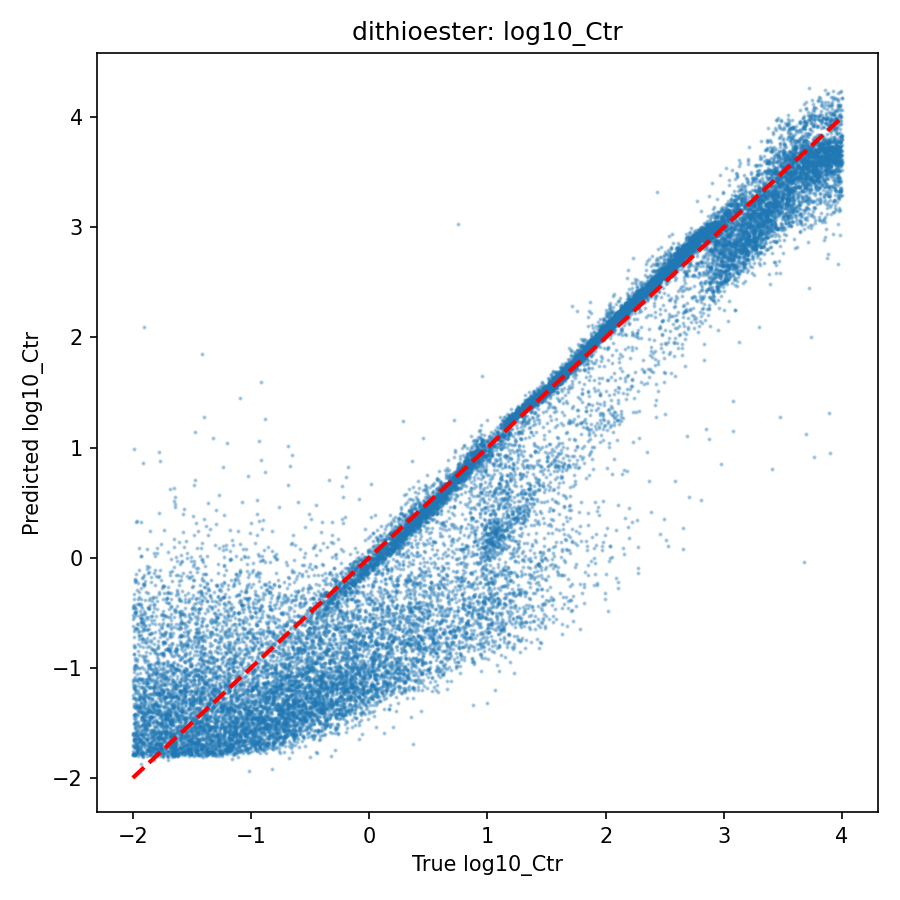
\includegraphics[width=0.32\linewidth]{../figures/parity_by_class/dithioester_log10_Ctr.png}
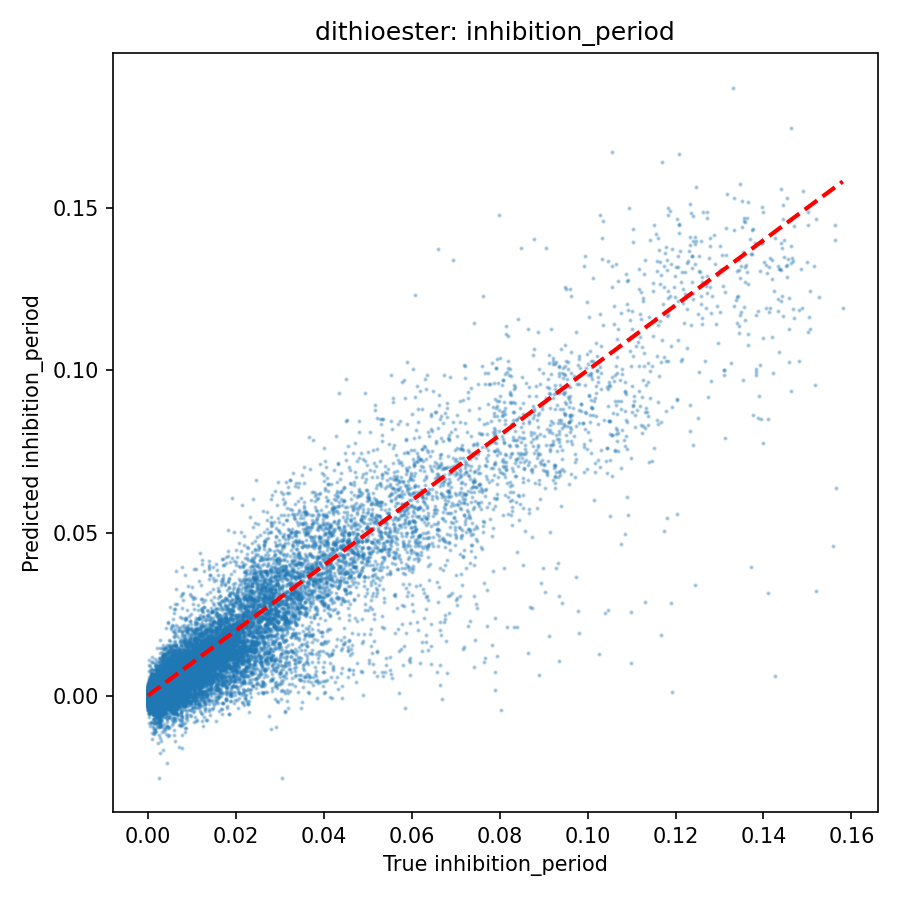
\includegraphics[width=0.32\linewidth]{../figures/parity_by_class/dithioester_inhibition_period.png}
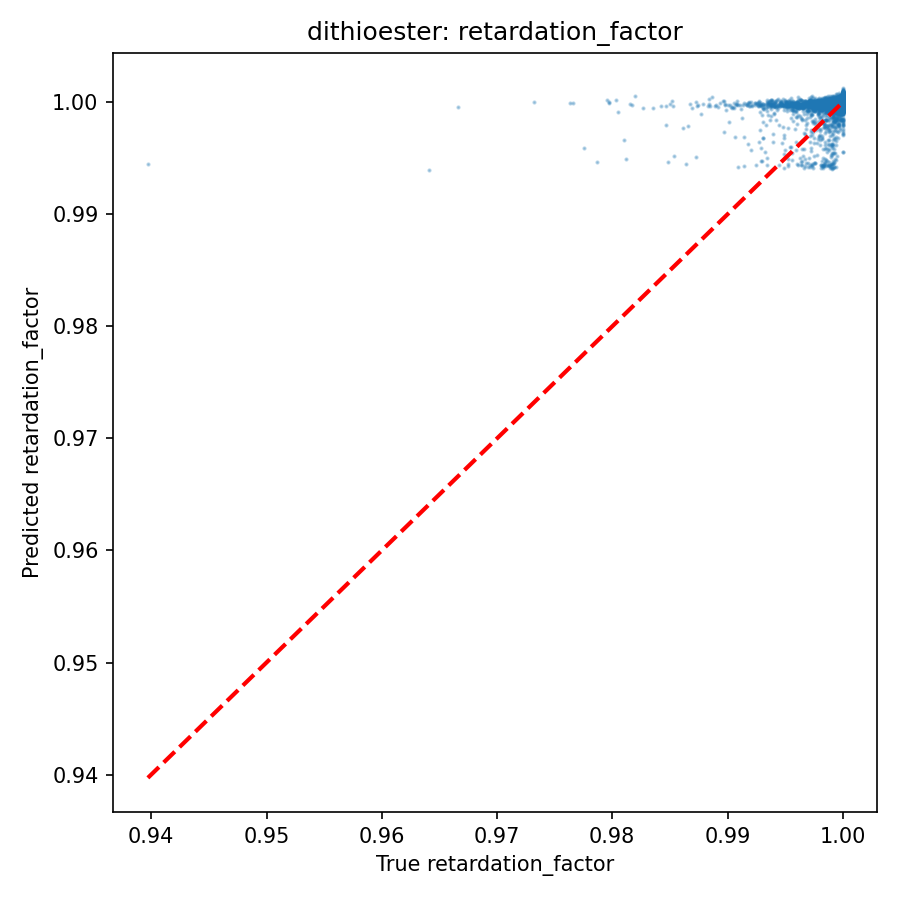
\includegraphics[width=0.32\linewidth]{../figures/parity_by_class/dithioester_retardation_factor.png}
\caption{Per-class parity plots for dithioester: (a) $\log_{10}(C_{\mathrm{tr}})$,
  (b) inhibition period, (c) retardation factor.}
\label{fig:parity_dithioester}
\end{figure}

\begin{figure}[htbp]
\centering
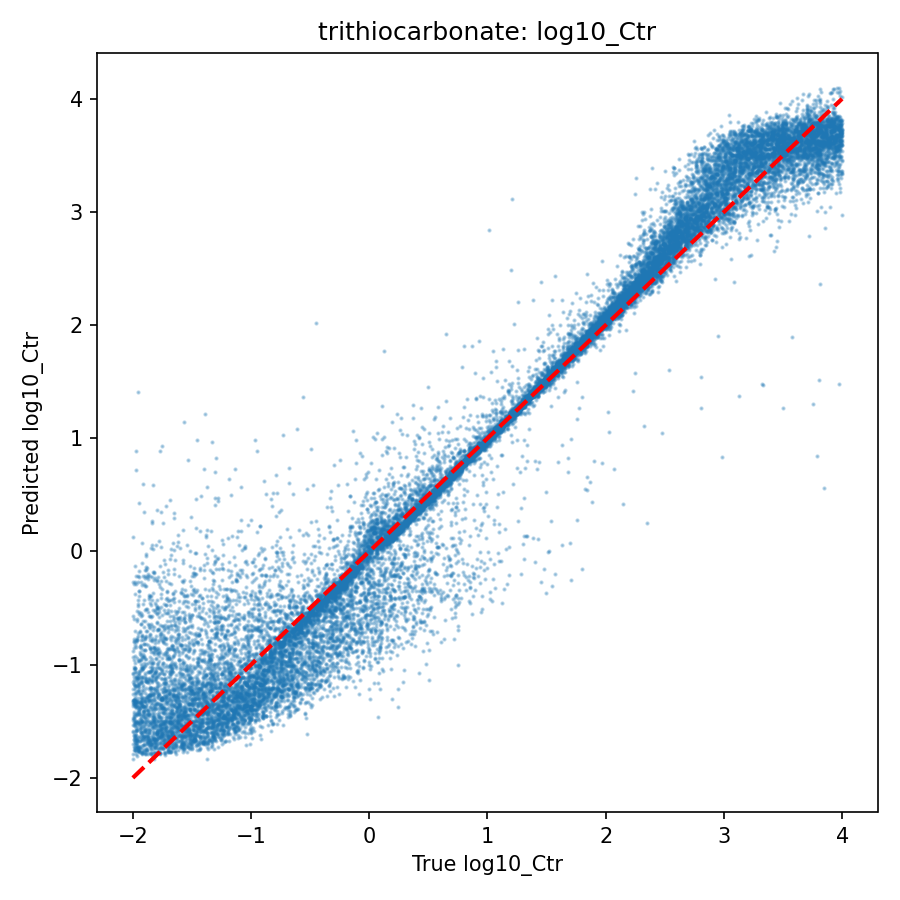
\includegraphics[width=0.32\linewidth]{../figures/parity_by_class/trithiocarbonate_log10_Ctr.png}
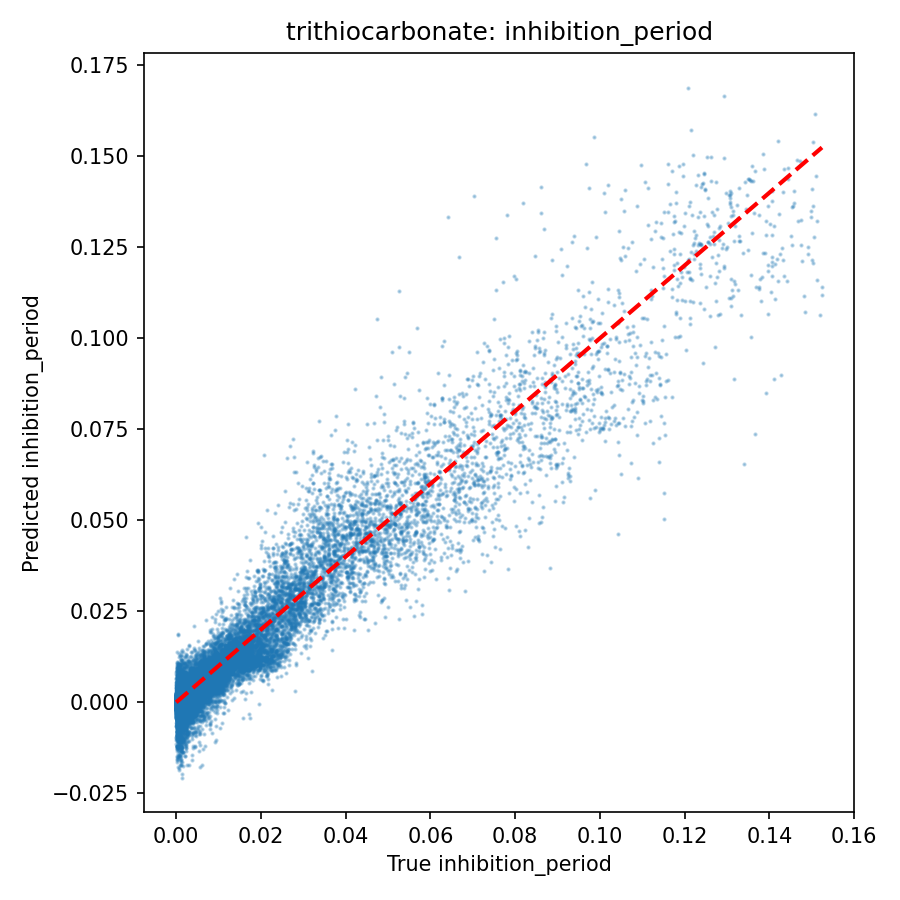
\includegraphics[width=0.32\linewidth]{../figures/parity_by_class/trithiocarbonate_inhibition_period.png}
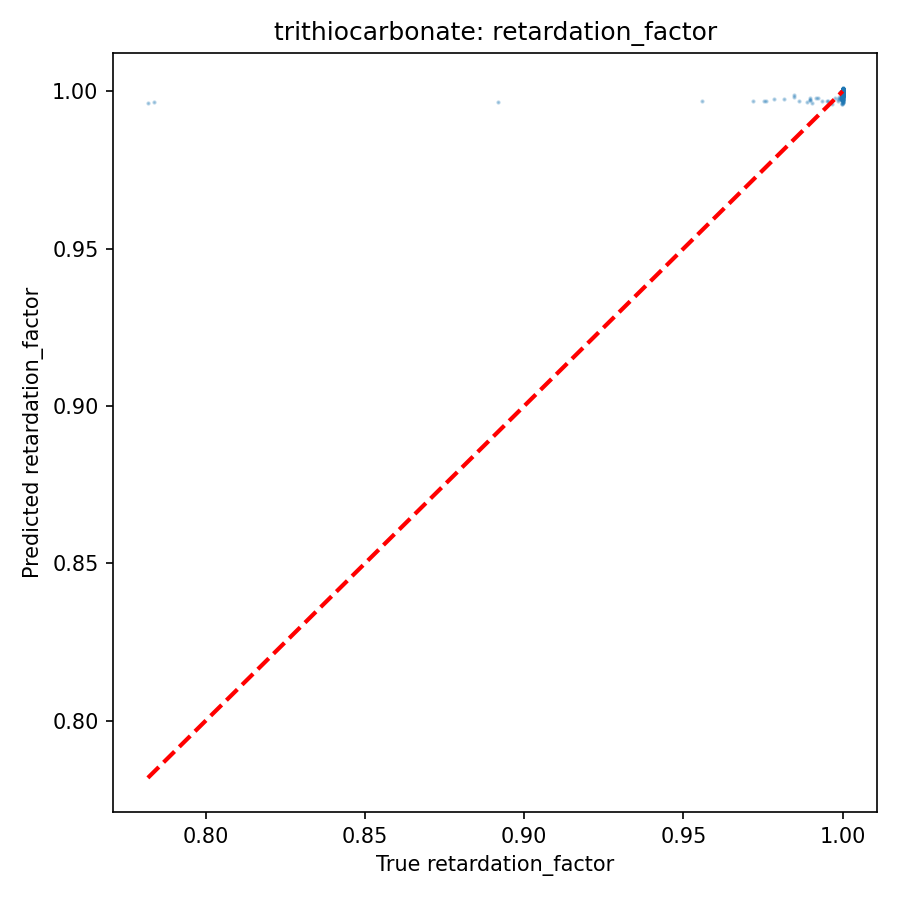
\includegraphics[width=0.32\linewidth]{../figures/parity_by_class/trithiocarbonate_retardation_factor.png}
\caption{Per-class parity plots for trithiocarbonate: (a) $\log_{10}(C_{\mathrm{tr}})$,
  (b) inhibition period, (c) retardation factor.}
\label{fig:parity_ttc}
\end{figure}

\begin{figure}[htbp]
\centering
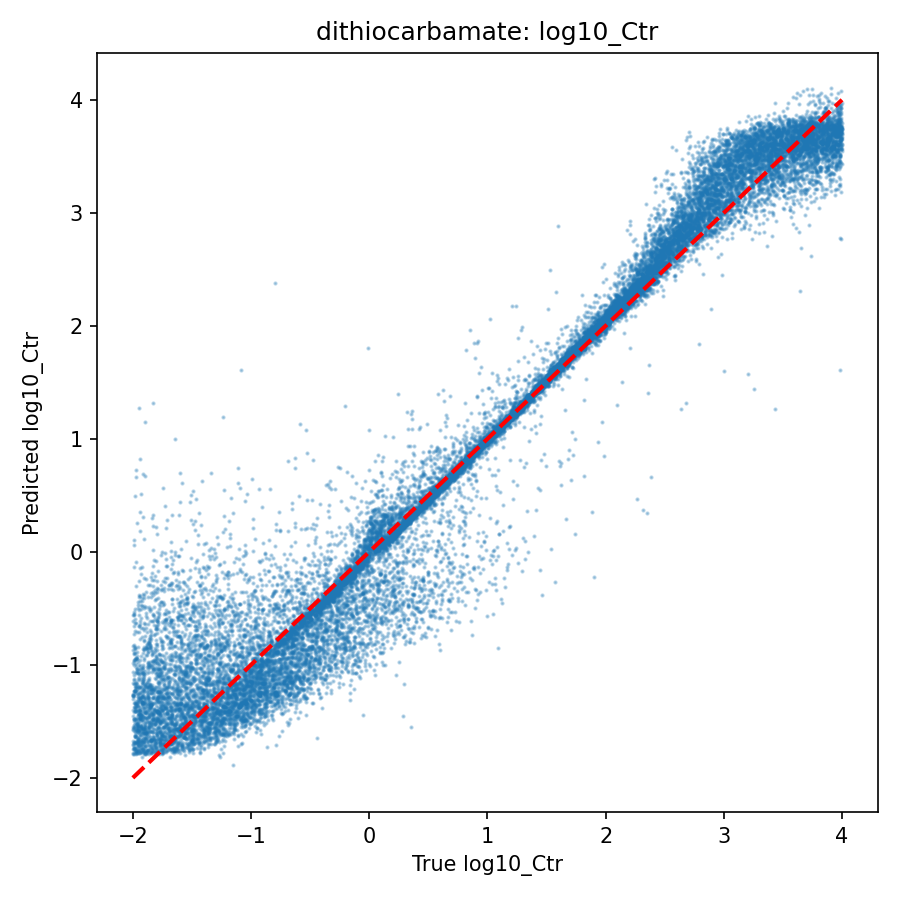
\includegraphics[width=0.32\linewidth]{../figures/parity_by_class/dithiocarbamate_log10_Ctr.png}
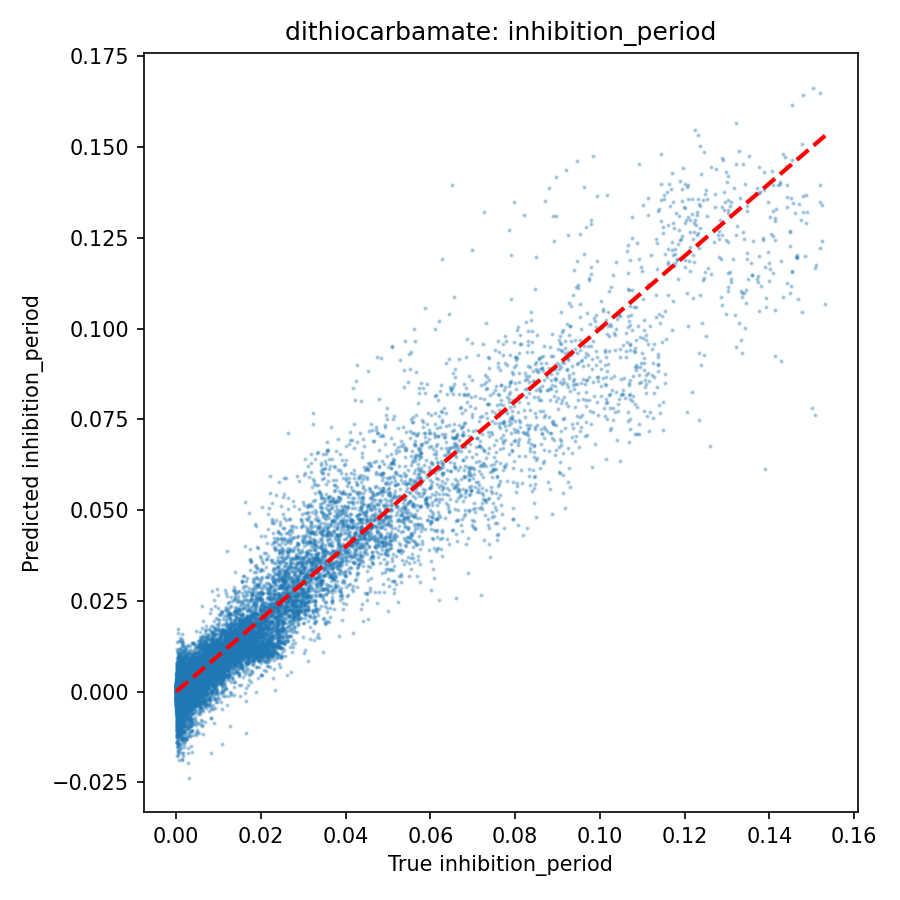
\includegraphics[width=0.32\linewidth]{../figures/parity_by_class/dithiocarbamate_inhibition_period.png}
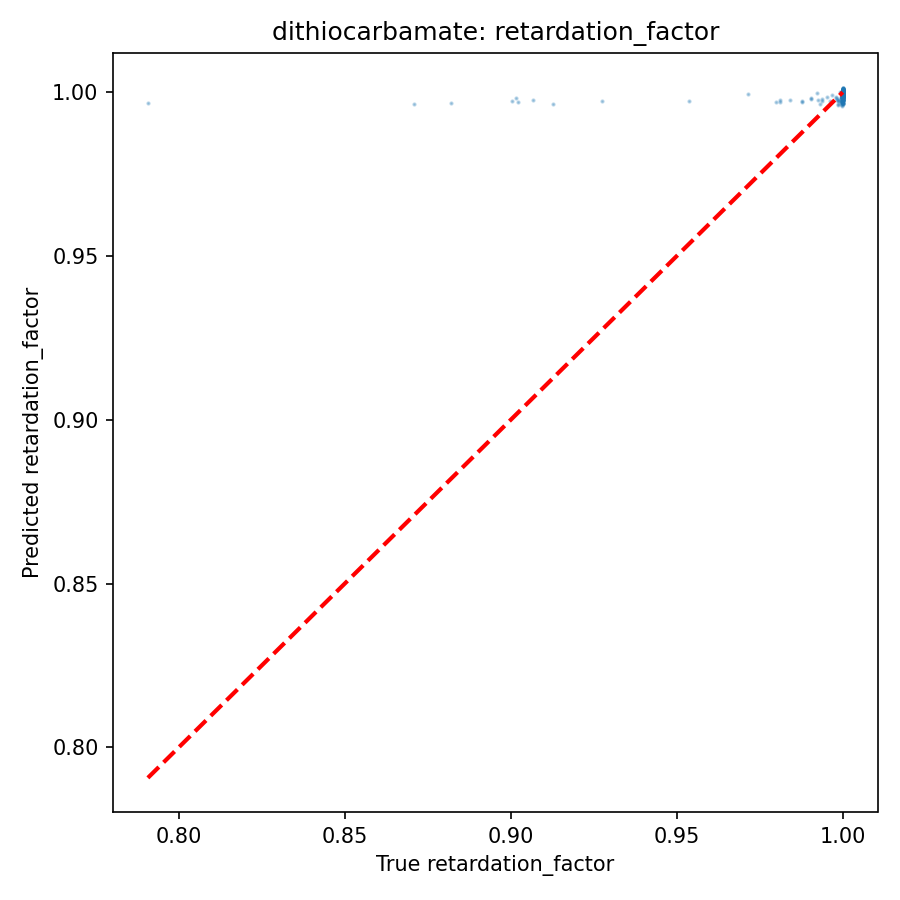
\includegraphics[width=0.32\linewidth]{../figures/parity_by_class/dithiocarbamate_retardation_factor.png}
\caption{Per-class parity plots for dithiocarbamate: (a) $\log_{10}(C_{\mathrm{tr}})$,
  (b) inhibition period, (c) retardation factor.}
\label{fig:parity_dithiocarbamate}
\end{figure}

\begin{figure}[htbp]
\centering
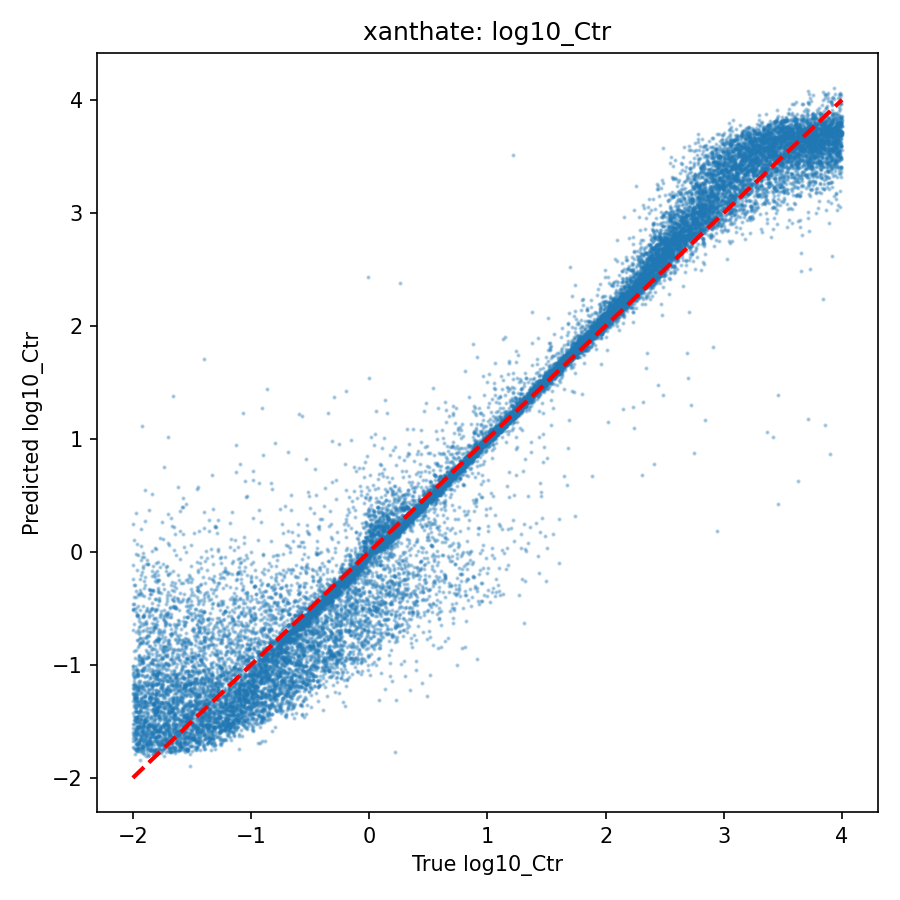
\includegraphics[width=0.32\linewidth]{../figures/parity_by_class/xanthate_log10_Ctr.png}
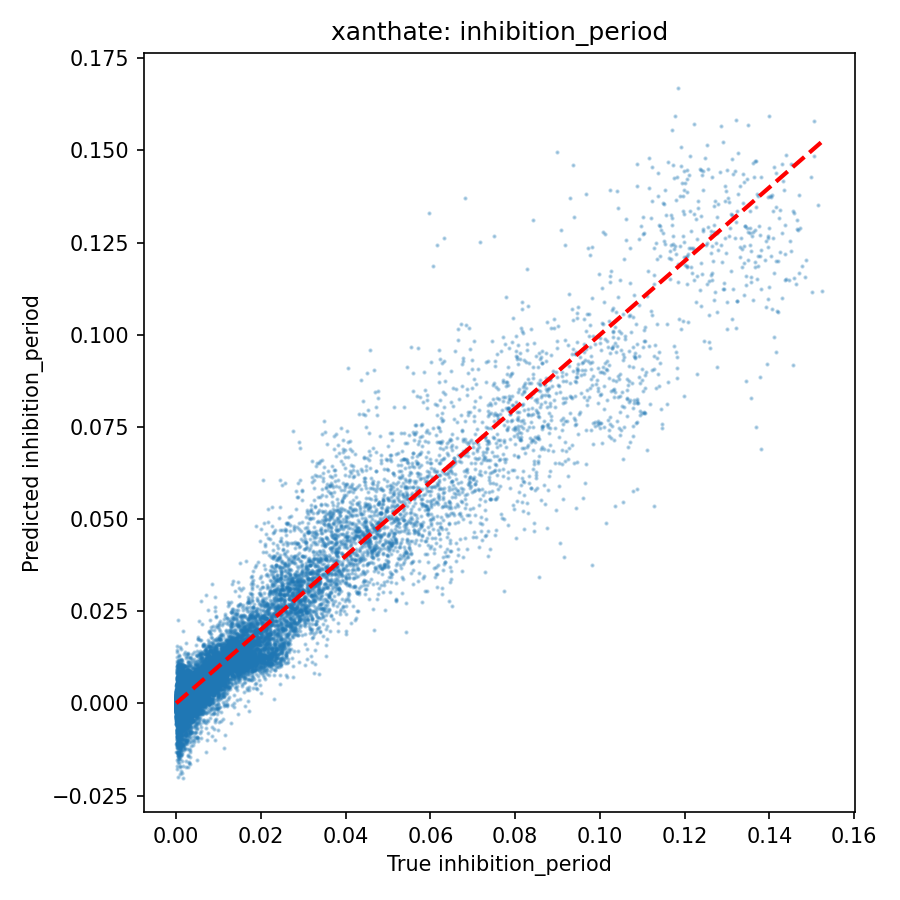
\includegraphics[width=0.32\linewidth]{../figures/parity_by_class/xanthate_inhibition_period.png}
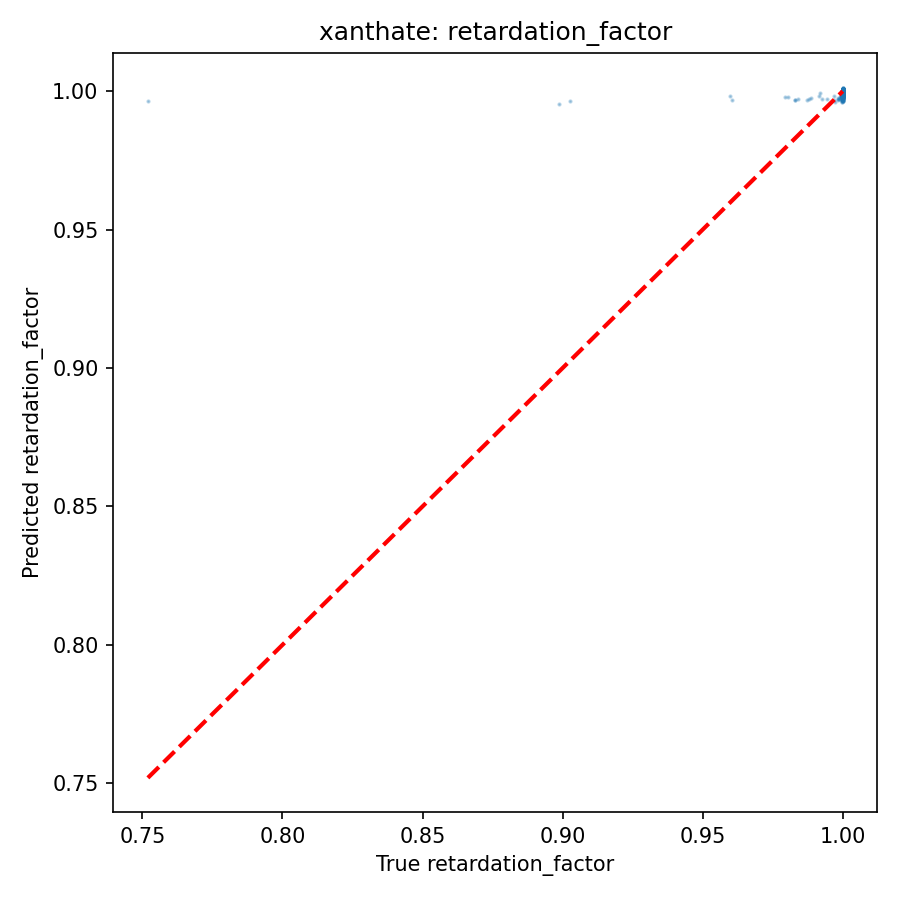
\includegraphics[width=0.32\linewidth]{../figures/parity_by_class/xanthate_retardation_factor.png}
\caption{Per-class parity plots for xanthate: (a) $\log_{10}(C_{\mathrm{tr}})$,
  (b) inhibition period, (c) retardation factor.}
\label{fig:parity_xanthate}
\end{figure}

\subsection{Residual Distributions}

Figures~\ref{fig:residuals} show the residual distributions for each output
parameter across the entire synthetic test set.

\begin{figure}[htbp]
\centering
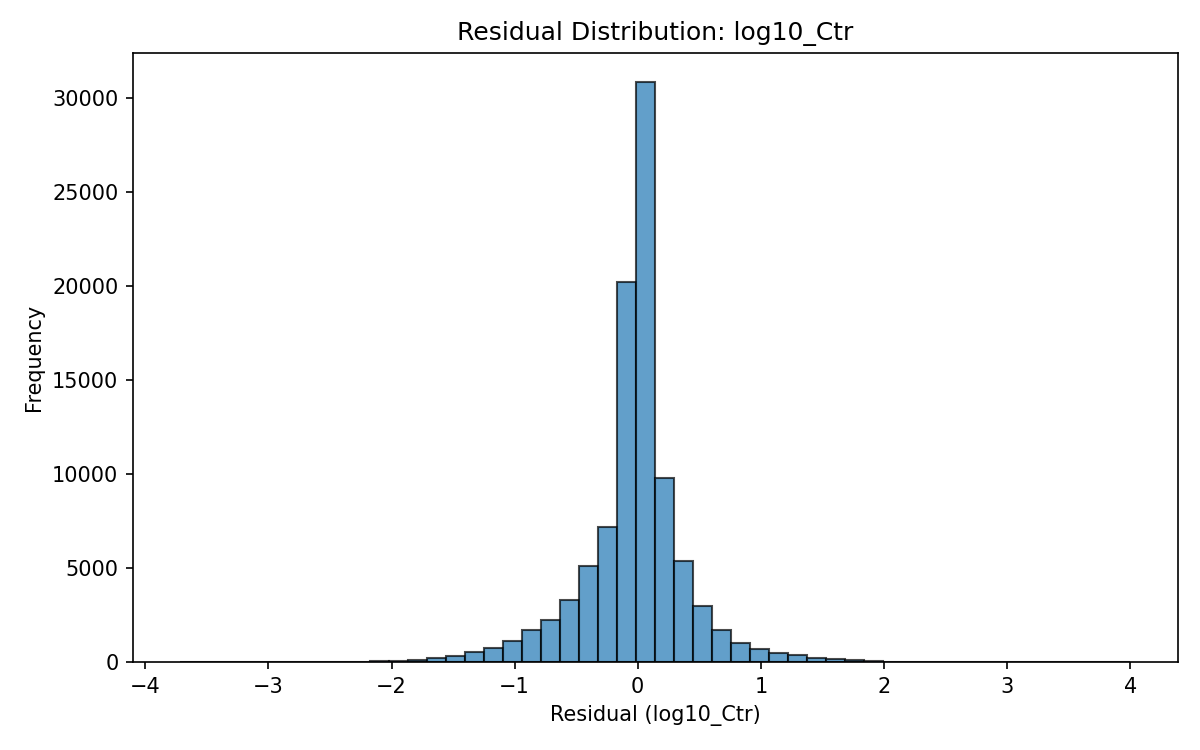
\includegraphics[width=0.32\linewidth]{../figures/residuals_log10_Ctr.png}
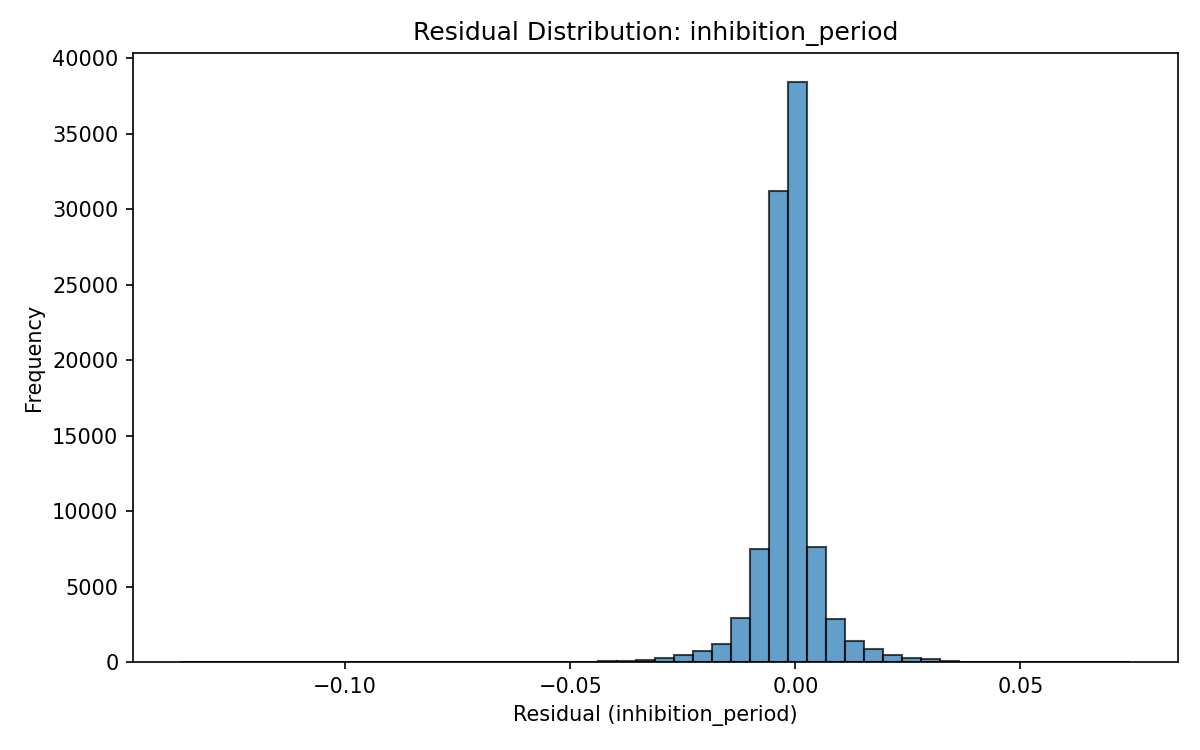
\includegraphics[width=0.32\linewidth]{../figures/residuals_inhibition_period.png}
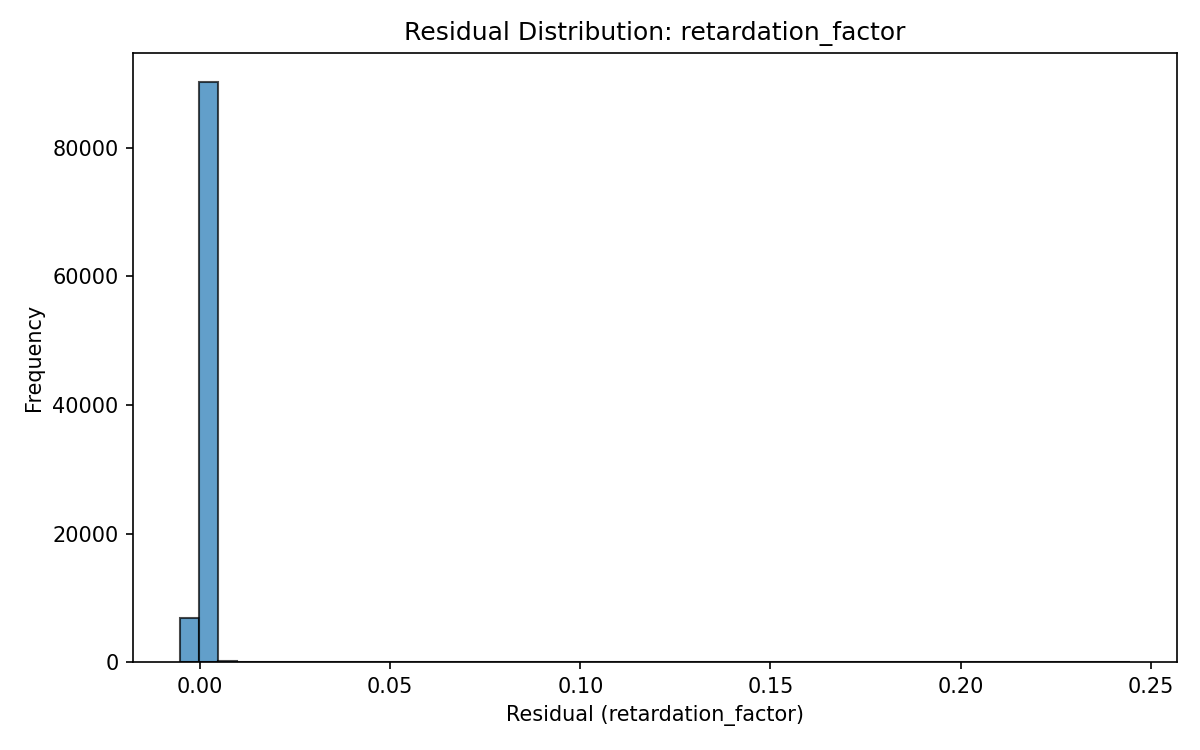
\includegraphics[width=0.32\linewidth]{../figures/residuals_retardation_factor.png}
\caption{Residual distributions on the synthetic test set:
  (a) $\log_{10}(C_{\mathrm{tr}})$, (b) inhibition period,
  (c) retardation factor.}
\label{fig:residuals}
\end{figure}

\end{document}
